%%%%%%%%%%%%%%%%%%%%%%%%%%%%%%%%%
%
%       EXERCÍCIO
%
%%%%%%%%%%%%%%%%%%%%%%%%%%%%%%%%%

\ifdefstring{\atividade}{prova}{%
    \ifdefstring{\modo}{objetivo}{%
        \renewcommand{\valorquestao}{\ValorQObj\ ponto}
    }{%
        \renewcommand{\valorquestao}{\ValorQDisc\ pontos}
    }%
}%

\begin{exercicioBanco}[\valorquestao]
Admita que um tipo de eucalipto tenha expectativa de crescimento exponencial, nos primeiros anos após seu plantio, modelado pela função
\[
y(t)=a^{\,t-1},
\]
na qual \(y\) representa a altura da planta em metros, \(t\) é considerado em anos, e \(a\) é uma constante maior que \(1\). O gráfico representa a função \(y\).

\begin{center}
    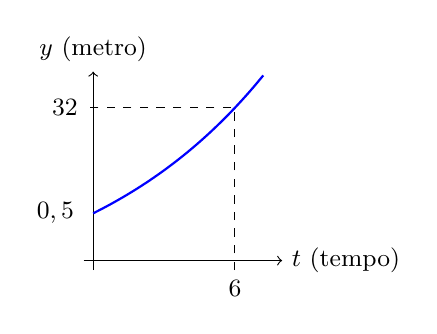
\begin{tikzpicture}[scale=1.2]

        % Eixos
        \draw[->] (-0.1,0) -- (2,0) node[right] {\small$t$ (tempo)};
        \draw[->] (0,-0.1) -- (0,2) node[above] {\small$y$ (metro)};

        % Gráfico de y = a^x (exponencial)
        \draw[domain=0:1.8, smooth, variable=\x, blue, thick] plot ({\x}, {exp(\x/2)-0.5});
        
        \draw node at (-0.4, 0.5) {\small\(0,5\)};
        \draw node at (1.5, -0.3) {\small\(6\)};
        \draw node at (-0.3, {exp(1.5/2)-0.5}) {\small\(32\)};
        
        \draw[dashed] (1.5, -0.1) -- (1.5,{exp(1.5/2)-0.5}) -- (-0.1, {exp(1.5/2)-0.5});
    \end{tikzpicture}
\end{center}

Admita ainda que \(y(0)\) fornece a altura da muda quando plantada, e deseja-se cortar os eucaliptos quando as mudas crescerem \(7,5\) m após o plantio. O tempo entre a plantação e o corte, em anos, é igual a:


% Define as alternativas
\newcommand{\alternativas}{%
    \begin{center}
        \begin{tabularx}{\textwidth}{XXXXX}
            (a) \(3\). &
            (b) \(4\). &
            (c) \(6\). &
            (d) \(8\). &
            (e) \(1\).
        \end{tabularx}
    \end{center}
}

% Define a resposta correta
\newcommand{\resposta}{B}

% Lógica condicional para exibição
\ifdefstring{\atividade}{lista}{%
    \alternativas
    \vspace{0.5em}
    
    \noindent\textbf{Resposta:} letra \textbf{\resposta}.
}{%
    \ifdefstring{\modo}{objetivo}{%
        \alternativas
    }{%
        % modo = discursiva → não mostra alternativas
    }
}
\end{exercicioBanco}

